\documentclass{article} % (short report)

%-- packages --
\usepackage{xcolor}
\usepackage{tabularx}
\usepackage{array}
\usepackage{graphicx}
\usepackage[section]{placeins}
\usepackage{booktabs} 
\usepackage{multirow} 
\usepackage{caption} 
\usepackage{subcaption}
\usepackage{listings}

%-- setup --
\newtheorem{theorem}{Teorema}
\newcolumntype{C}{>{\centering\arraybackslash}X}
\graphicspath{ {./} }

\title{Forma Normale Congiuntiva}
\author{Tescaro Rocco}
\date{\today}

%-- document --
\begin{document}

\thispagestyle{plain}
\begin{center}
    \Large
    \textbf{Forma Normale Congiuntiva}
    
    \vspace{0.2cm}
    \large
    B003725 Intelligenza Artificiale (2023/24)
    
    \vspace{0.4cm}
    \textbf{Tescaro Rocco}
    \vspace{0.2cm}
\end{center}

\begin{abstract}
    
In questo esercizio si generalizza e implementa (in un linguaggio di programmazione a scelta) la procedura descritta nella sezione 7.5.2 di R\&N 2021 per convertire una generica formula in logica proposizionale in forma normale congiuntiva (CNF). Il programma deve accettare una stringa nel linguaggio descritto nella figura 7.7 del libro, e produrre in output la corrispondente formula in CNF.

\end{abstract}

\section*{Introduzione} 

Come dichiarato nella sezione precedente, l'obbiettivo di questo progetto è quello di implementare un algoritmo che converta una formula in logica proposizionale, nello specifico da Backus-Naur Form (BNF) a Conjunctive Normal Form (CNF).

Si deve inoltre implementare un sistema di verifica della correttezza della sintassi della formula in BNF, in modo da garantire che l'algoritmo di conversione possa operare correttamente. Non direttamente richiesto, è stato implementato anche un sistema di generazione casuale di formule in BNF, per testare l'algoritmo di conversione.

In seguito riportata la formalizzazione del metalinguaggio di una BNF in "Artificial Intelligence: A Modern Approach (R\&N 2021)":

\begin{figure}[htbp]
    \caption{\textbf{BNF Syntax}}
    \centering
    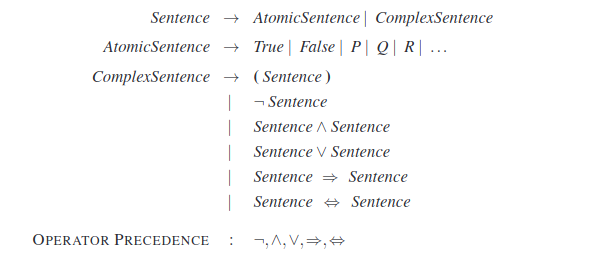
\includegraphics[width=\linewidth]{bnf}
\end{figure}

E' necessario precisare che per le Atomic Sentences non è stata limitata la scelta dei simboli ma il programma accetta qualsiasi stringa alfanumerica che non contenga spazi e non concida con altri operatori, inoltre per semplificare la scrittura delle formule gli operatori di negazione, congiunzione, disgiunzione, implicazione e doppia implicazione sono stati sostituiti con i simboli '!', '\&', '$|$', '$=>$' e '$<=>$' rispettivamente.
Poichè non è l'obbiettivo del progetto, e al fine di esemplificare il partizionamento delle stringhe, ogni operatore è stato distanziato da uno spazio.
Per le formule in CNF sono state prese le medesime scelte. 
Per quanto riguarda invece la procedura descritta nel capitolo 7.5.2 di R\&N 2021, essa è stata implementata seguendo i passaggi descritti nel libro, senza quindi apportare ottimizzazioni o modifiche, adottando però una struttura dati che permettesse di eseguire ugualmente le operazioni in modo efficiente.

\begin{figure}[htbp]
    \caption{\textbf{CNF Conversion}}
    \centering
    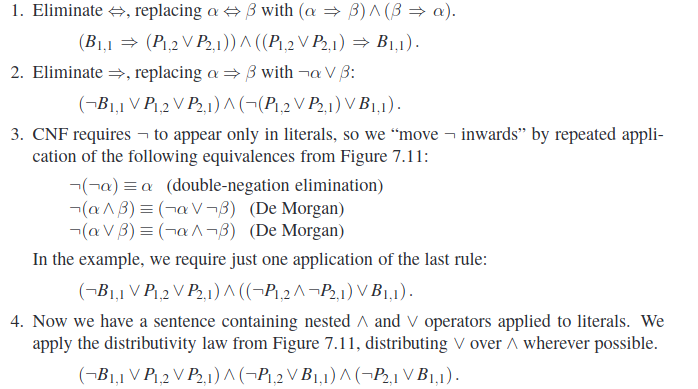
\includegraphics[width=\linewidth]{cnf}
\end{figure}


\section*{Implementazione}  

Il primo problema che è stato affrontato è quello della verifica della correttezza della sintassi della formula in BNF. Per farlo è stato implementato un parser che, dato in input una stringa, la suddivide in token e verifica che la sequenza di token sia corretta.
L'algoritmo è ricorsivo e verifica che ciascun contenuto tra parentesi sia corretto, ovvero che sia una formula ben formata, in caso contrario restituisce un errore.
Una volta validata una stringa è necessario convertirla in una struttura dati su cui sia facile operare. 

\vspace{0.5cm}

\begin{tabular}{|p{5cm}|p{5cm}|}
    \textbf{Sentence} & \textbf{Result} \\ \hline
    ( A \& B ) $|$ C \& D $<=>$ E & True \\
    ( A \& B ) $|$ \& D $<=>$ E ! & False \\
\end{tabular}

\vspace{0.5cm}

La struttura dati scelta per rappresentare la formula è un albero binario, noto come \textbf{Expression Tree}. In un Expression Tree, ogni nodo interno rappresenta un operatore logico e i suoi figli rappresentano gli operandi, che possono essere a loro volta formule o "Atomic Sentence" (le foglie dell'albero). Ogni nodo ha quattro attributi: il simbolo dell'operatore, il figlio sinistro, il figlio destro e il genitore. Per gli operatori unari, come la negazione, il figlio destro è nullo. Per le atomic sentence, il simbolo dell'operatore è il simbolo della variabile e i figli sono nulli.

L'algoritmo di costruzione dell'albero è ricorsivo e opera in tre fasi:

\begin{itemize}
    \item \textbf{Tokenizzazione}: la stringa che rappresenta la formula viene convertita in una lista di token.
    \item \textbf{Ordinamento}: i token vengono ordinati secondo l'algoritmo di \textbf{shouting yard}, che rispetta le precedenze degli operatori.
    \item \textbf{Costruzione dell'albero}: l'albero viene costruito ricorsivamente a partire dal token con la precedenza più bassa, procedendo verso i token con precedenza più alta.
\end{itemize}

\vspace{0.5cm}

\begin{tabular}{|p{4.5cm}|p{5.5cm}|}
    \textbf{Sentence} & \textbf{Result} \\ \hline
    ( A \& B ) $|$ C \& D $<=>$ E & ( ( ( A \& B ) $|$ ( C \& D ) ) $<=>$ E ) \\
\end{tabular}

\vspace{0.5cm}

\noindent Una volta costruito l'albero è possibile procedere con la conversione in CNF. L'algoritmo di conversione ripercorre, come già detto, i passaggi descritti nel libro (vedi sezione precedente).
Ciascuno di questi sottopassaggi è implementato con un attraversamento preorder dell'albero con una leggera variazione per l'ultimo passaggio, in cui l'attraversamento è sempre preorder ma, in caso si fossero effettuate le modifiche, e si verificasse una situazione favorevole con il nodo genitore, l'algoritmo ritorna al nodo genitore e ripete il passaggio.
Per questo motivo la complessià dell'algoritmo è equivalente a circa 4 volte la complessità di un attraversamento preorder dell'albero ovvero O(n) con n il numero di nodi (nel nostro caso operatori più variabili). Poichè non particolarmente utile al resto del codice la proprietà genitore di ciascun nodo non è stata mantenuta durante le varie operazioni (anche se sarebbe stato possibile) e questo porta ad un ulteriore attraversamente, in questo caso inorder, per ristabilire la proprietà prima di poter effettuare l'ultimo passaggio.
Poichè abbiamo adottato una struttura ad albero è stata infine implementata un'ulterio funzione che stampa l'albero semplificando le parentesi (altrimenti aggiunte per ogni operazione binaria) e mostrando così la formula in un'effettiva CNF.

\vspace{0.5cm}

\begin{tabular}{|p{3cm}|p{7cm}|}
    \footnotesize \textbf{Sentence} & \footnotesize ( A \& B ) $|$ ( C \& D ) \\
    \footnotesize \textbf{Tree} & \footnotesize ( ( A \& B ) $|$ ( C \& D ) ) \\
    \footnotesize \textbf{CNF (unsimplified)} & \footnotesize ( ( ( C $|$ A ) \& ( D $|$ A ) ) \& ( ( C $|$ B ) \& ( D $|$ B ) ) ) \\
    \footnotesize \textbf{CNF (simplified)} & \footnotesize ( C $|$ A ) \& ( D $|$ A ) \& ( C $|$ B ) \& ( D $|$ B ) \\
\end{tabular}

\vspace{0.5cm}

\section*{Test} 

L'implementazione dell'algoritmo è stata realizzata in linguaggio Python 3.9.7. Il codice è stato scritto e testato su una macchina le cui specifiche sono riportate in appendice.
I test eseguiti pongono come obiettivo verificare che la validazione della sintassi della formula in BNF sia corretta su un insieme casuale di formule ben formate. Per questo motivo sono state implementate tre altre funzioni: la prima si occupa di generare bnf casuali prendendo come input il numero di variabili, il numero di ripetizioni e la probabilità associata a ciascun operatore, la seconda esegue la funzione di validazione su un insieme di dimensione arbitraria di formule bnf casuali e l'utente può decidere se generane di corrette o meno (nel secondo caso viene semplicemente sostituita una parentesi o una variabile con un operatore) e la terza esegue la conversione in CNF data in input una formula bnf.
La funzione che si occupa di generare bnf casuali opera similiarmente all'algoritmo che costruisce l'expression tree, scegliendo un operatore casuale fino a raggiungere il numero di variabili impostato, gli operatori binari chiameranno ricorsivamente la funzione operando su metà delle variabili disponibili, gli operatori unari su tutte le variabili ancora disponibili. Non è stato impostato un effettivo limite al numero di operatori, tuttavia per limitare la dimensione della stringa finale (che a causa dell'operatore unario potrebbe essere illimitata) la probabilità associata all'operatore di negazione è stata impostata al 10\%.
Le funzioni descritte sono state chiamate per un numero di 100 formule casuali, ciascuna con tre variabili e due ripetizioni, sia per quelle ben formate che per quelle non ben formate. Inoltre durante la fase di sviluppo sono state eseguiti diversi test su formule specifiche per verificare casi limiti e garantire la correttezza degli algoritmi.

\section*{Conclusioni}  

L'algoritmo di conversione in CNF è stato testato con successo su un set di formule casuali, dimostrando la sua efficacia. Tuttavia, sono possibili alcuni miglioramenti futuri:

- Migliorare il sistema di parsing togliendo la regola implicita che impone la presenza di spazi tra gli operatori.

- Mantenere l'attributo "parent" durante le varie operazioni.

- Implementare l'algoritmo in un linguaggio di programmazione specifico per ottimizzare le prestazioni.

- Eseguire test più approfonditi per identificare eventuali errori non rilevati nei test precedenti.


\vfill
\noindent\makebox[\linewidth]{\rule{\textwidth}{0.01pt}}
\footnotesize
appendice:

specifiche hardware e software
\centering
\begin{tabularx}{\textwidth}{|>{\hsize=2.\hsize}C|*{4}{>{\hsize=0.5\hsize}C|}}
    \hline
     \textbf{Processor} & \textbf{RAM} & \textbf{System type} & \textbf{OS distro} & \textbf{OS version} \\
     \hline
     AMD Ryzen 7 5700U with Radeon Graphics 1.80 GHz & 16.0 GB & 64-bit & Linux & Arch \\
     \hline
\end{tabularx}

\end{document}
